\section{More on tableaus, their representations and their properties}

\subsection{Preliminaries: On subsets and subformulas}

In this subsection, we present two lemmas on subsets and subformulas. Given a formula \(\phi\), a subformula is a substring of \(\phi\) that is also a formula.

\begin{lemma}
    A set \(S\) of cardinality \(n\) has \(2^n\) subsets.
\end{lemma}
\begin{proof}
    To construct a subset \(S' \subseteq S\), each element of \(S\) can either appear or not appear in \(S'\). This involves a total of \(n\) independent binary choices. Hence, there are \(2^n\) possible subsets.
\end{proof}

\begin{lemma}
    A formula \(\phi\) has at most \(\abs{\phi}\) subformulas.
\end{lemma}
\begin{proof}
    Consider the parse tree of \(\phi\), where every node contains exactly one symbol and is the root of a subtree that represents a subformula of \(\phi\). Hence we have
    %
    \begin{align*}
        & \text{Number of subformulas of } \phi\\
        =\;& \text{Number of nodes in parse tree of } \phi\\
        =\;& \text{Number of symbols that appear in parse tree of } \phi\\
        \leq\;& \text{Number of symbols in } \phi \tag{as brackets do not appear in parse trees}\\
        =\;& \abs{\phi}\text{.} \qedhere
    \end{align*}
\end{proof}

\subsection{Tableaus as lists of theories}

While tableaus can be visualised as trees, they can also be represented as lists. To see how this works, let us first review the \(\alpha\)- and \(\beta\)- rules. As shown in tables \ref{tab:Ch05-alpha-rules} and \ref{tab:Ch05-beta-rules}, each \(\alpha\)-rule produces at most two new nodes \(\alpha_1\) and \(\alpha_2\), while each \(\beta\)-rule produces at most two new nodes \(\beta_1\) and \(\beta_2\).

\begin{table}[H]
    \centering
    \begin{tabular}{|c|cc|}
        \hline
        \(\alpha\) & \(\alpha_1\) & \(\alpha_2\)\\
        \hline
        \((A\land B)\) & \(A\) & \(B\)\\
        \hline
        \(\neg(A\lor B)\) & \(\neg A\) & \(\neg B\)\\
        \hline
        \(\neg(A\rightarrow B)\) & \(A\) & \(\neg B\)\\
        \hline
        \(\neg\neg A\) & \(A\) & -\\
        \hline
    \end{tabular}

    \caption{The \(\alpha\)-rules tabulated.}
    \label{tab:Ch05-alpha-rules}
\end{table}

\begin{table}[H]
    \centering
    \begin{tabular}{|c|cc|}
        \hline
        \(\beta\) & \(\beta_1\) & \(\beta_2\)\\
        \hline
        \((A\lor B)\) & \(A\) & \(B\)\\
        \hline
        \((A\rightarrow B)\) & \(\neg A\) & \(B\)\\
        \hline
        \(\neg(A\land B)\) & \(\neg A\) & \(\neg B\)\\
        \hline
    \end{tabular}

    \caption{The \(\beta\)-rules tabulated.}
    \label{tab:Ch05-beta-rules}
\end{table}


Instead of a tree, we represent a tableau as a list of \emph{theories}, where each theory is a set of unticked formulas in a branch that has not yet closed. Figure \ref{fig:Ch05-tableau-as-list}, based on Figure \ref{fig:Ch03-satisfiability-tableau}, shows the construction of a propositional tableau in both tree and list form.


\begin{figure}[H]
    \centering
    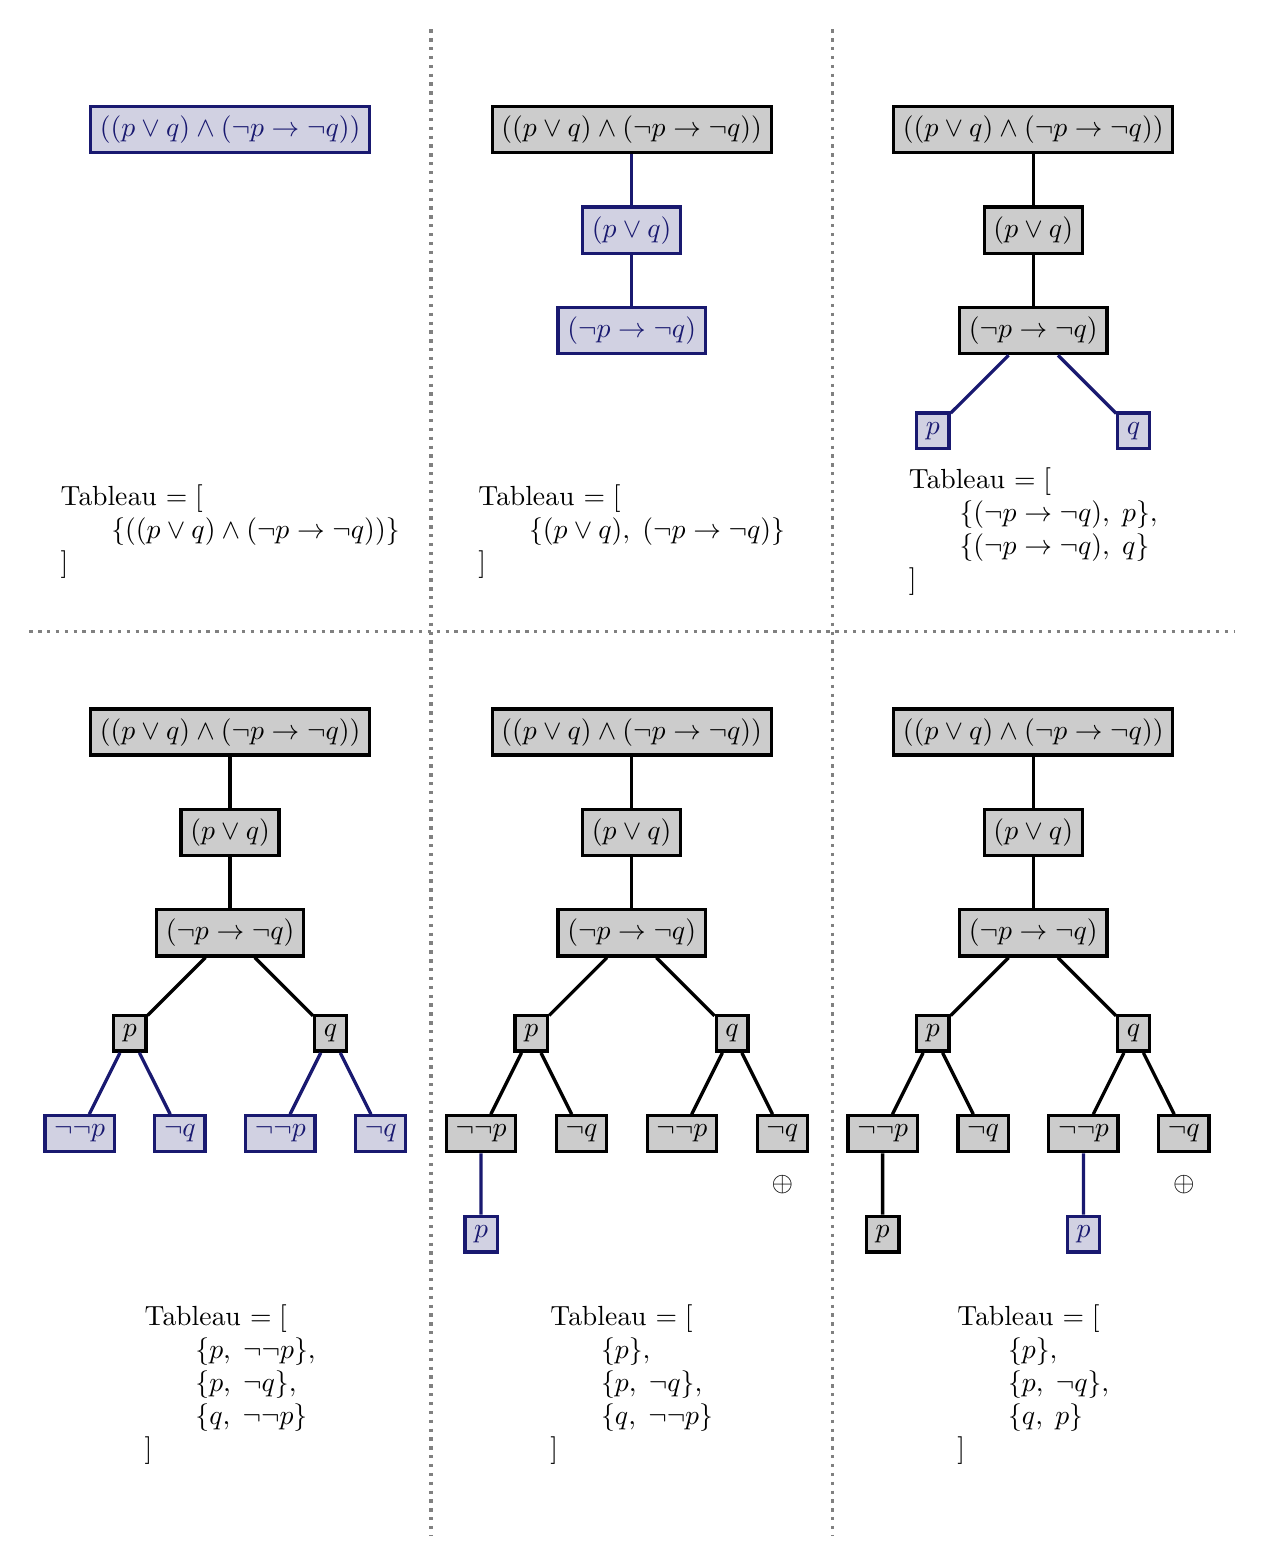
\begin{tikzpicture}[scale=1.275]
        \begin{scope}[shift={(0, 0)}]
            \node (0) at (0, 0)[draw=MidnightBlue, very thick, MidnightBlue, fill=MidnightBlue!20] {\(((p \lor q) \land (\neg p \rightarrow \neg q))\)};

            \node at (0, -4) [black, align=left]{
                Tableau \(= [\)\\
                \hspace{1.5em} \(\{((p \lor q) \land (\neg p \rightarrow \neg q))\}\)\\
                \(]\)
            };
        \end{scope}

        \begin{scope}[shift={(4, 0)}]
            \node (0) at (0, 0)[draw=black, very thick, fill=black!20] {\(((p \lor q) \land (\neg p \rightarrow \neg q))\)};
            \node[right of=0, xshift=30pt] {\checkmark};

            \node (1) at (0, -1)[draw=MidnightBlue, very thick, MidnightBlue, fill=MidnightBlue!20] {\((p \lor q)\)};

            \node (2) at (0, -2)[draw=MidnightBlue, very thick, MidnightBlue, fill=MidnightBlue!20] {\((\neg p \rightarrow \neg q)\)};

            \draw[MidnightBlue, very thick] (0) -- (1) -- (2);

            \node at (0, -4) [black, align=left]{
                Tableau \(= [\)\\
                \hspace{1.5em} \(\{(p \lor q),\; (\neg p \rightarrow \neg q)\}\)\\
                \(]\)
            };
        \end{scope}

        \begin{scope}[shift={(8, 0)}]
            \node (0) at (0, 0)[draw=black, very thick, fill=black!20] {\(((p \lor q) \land (\neg p \rightarrow \neg q))\)};
            \node[right of=0, xshift=30pt] {\checkmark};

            \node (1) at (0, -1)[draw=black, very thick, fill=black!20] {\((p \lor q)\)};
            \node[right of=1] {\checkmark};

            \node (2) at (0, -2)[draw=black, very thick, fill=black!20] {\((\neg p \rightarrow \neg q)\)};

            \node (3) at (-1, -3)[draw=MidnightBlue, very thick, MidnightBlue, fill=MidnightBlue!20] {\(p\)};

            \node (4) at (1, -3)[draw=MidnightBlue, very thick, MidnightBlue, fill=MidnightBlue!20] {\(q\)};

            \draw[black, very thick] (0) -- (1) -- (2);
            \draw[MidnightBlue, very thick] (2) -- (3);
            \draw[MidnightBlue, very thick] (2) -- (4);

            \node at (0, -4) [black, align=left]{
                Tableau \(= [\)\\
                \hspace{1.5em} \(\{(\neg p \rightarrow \neg q),\; p\},\)\\
                \hspace{1.5em} \(\{(\neg p \rightarrow \neg q),\; q\}\)\\
                \(]\)
            };
        \end{scope}

        \begin{scope}[shift={(0, -6)}]
            \node (0) at (0, 0)[draw=black, very thick, fill=black!20] {\(((p \lor q) \land (\neg p \rightarrow \neg q))\)};
            \node[right of=0, xshift=30pt] {\checkmark};

            \node (1) at (0, -1)[draw=black, very thick, fill=black!20] {\((p \lor q)\)};
            \node[right of=1] {\checkmark};

            \node (2) at (0, -2)[draw=black, very thick, fill=black!20] {\((\neg p \rightarrow \neg q)\)};
            \node[right of=2, xshift=10pt] {\checkmark};

            \node (3) at (-1, -3)[draw=black, very thick, fill=black!20] {\(p\)};

            \node (4) at (1, -3)[draw=black, very thick, fill=black!20] {\(q\)};

            \node (5) at (-1.5, -4)[draw=MidnightBlue, very thick, MidnightBlue, fill=MidnightBlue!20] {\(\neg\neg p\)};

            \node (6) at (-0.5, -4)[draw=MidnightBlue, very thick, MidnightBlue, fill=MidnightBlue!20] {\(\neg q\)};

            \node (7) at (0.5, -4)[draw=MidnightBlue, very thick, MidnightBlue, fill=MidnightBlue!20] {\(\neg\neg p\)};

            \node (8) at (1.5, -4)[draw=MidnightBlue, very thick, MidnightBlue, fill=MidnightBlue!20] {\(\neg q\)};

            \draw[black, very thick] (0) -- (1) -- (2);
            \draw[black, very thick] (2) -- (3);
            \draw[black, very thick] (2) -- (4);
            \draw[MidnightBlue, very thick] (3) -- (5);
            \draw[MidnightBlue, very thick] (3) -- (6);
            \draw[MidnightBlue, very thick] (4) -- (7);
            \draw[MidnightBlue, very thick] (4) -- (8);

            \node at (0, -6.5) [black, align=left]{
                Tableau \(= [\)\\
                \hspace{1.5em} \(\{p,\; \neg\neg p\},\)\\
                \hspace{1.5em} \(\{p,\; \neg q\},\)\\
                \hspace{1.5em} \(\{q,\; \neg\neg p\}\)\\
                \(]\)
            };
        \end{scope}

        \begin{scope}[shift={(4, -6)}]
            \node (0) at (0, 0)[draw=black, very thick, fill=black!20] {\(((p \lor q) \land (\neg p \rightarrow \neg q))\)};
            \node[right of=0, xshift=30pt] {\checkmark};

            \node (1) at (0, -1)[draw=black, very thick, fill=black!20] {\((p \lor q)\)};
            \node[right of=1] {\checkmark};

            \node (2) at (0, -2)[draw=black, very thick, fill=black!20] {\((\neg p \rightarrow \neg q)\)};
            \node[right of=2, xshift=10pt] {\checkmark};

            \node (3) at (-1, -3)[draw=black, very thick, fill=black!20] {\(p\)};

            \node (4) at (1, -3)[draw=black, very thick, fill=black!20] {\(q\)};

            \node (5) at (-1.5, -4)[draw=black, very thick, fill=black!20] {\(\neg\neg p\)};
            \node[above left of=5, xshift=15pt, yshift=-5pt] {\checkmark};

            \node (6) at (-0.5, -4)[draw=black, very thick, fill=black!20] {\(\neg q\)};

            \node (7) at (0.5, -4)[draw=black, very thick, fill=black!20] {\(\neg\neg p\)};

            \node (8) at (1.5, -4)[draw=black, very thick, fill=black!20] {\(\neg q\)};
            \node [below of=8, yshift=10pt] {\(\oplus\)};
            
            \node (9) at (-1.5, -5)[draw=MidnightBlue, very thick, MidnightBlue, fill=MidnightBlue!20] {\(p\)};

            \draw[black, very thick] (0) -- (1) -- (2);
            \draw[black, very thick] (2) -- (3);
            \draw[black, very thick] (2) -- (4);
            \draw[black, very thick] (3) -- (5);
            \draw[black, very thick] (3) -- (6);
            \draw[black, very thick] (4) -- (7);
            \draw[black, very thick] (4) -- (8);
            \draw[MidnightBlue, very thick] (5) -- (9);

            \node at (0, -6.5) [black, align=left]{
                Tableau \(= [\)\\
                \hspace{1.5em} \(\{p\},\)\\
                \hspace{1.5em} \(\{p,\; \neg q\},\)\\
                \hspace{1.5em} \(\{q,\; \neg\neg p\}\)\\
                \(]\)
            };
        \end{scope}

        \begin{scope}[shift={(8, -6)}]
            \node (0) at (0, 0)[draw=black, very thick, fill=black!20] {\(((p \lor q) \land (\neg p \rightarrow \neg q))\)};
            \node[right of=0, xshift=30pt] {\checkmark};

            \node (1) at (0, -1)[draw=black, very thick, fill=black!20] {\((p \lor q)\)};
            \node[right of=1] {\checkmark};

            \node (2) at (0, -2)[draw=black, very thick, fill=black!20] {\((\neg p \rightarrow \neg q)\)};
            \node[right of=2, xshift=10pt] {\checkmark};

            \node (3) at (-1, -3)[draw=black, very thick, fill=black!20] {\(p\)};

            \node (4) at (1, -3)[draw=black, very thick, fill=black!20] {\(q\)};

            \node (5) at (-1.5, -4)[draw=black, very thick, fill=black!20] {\(\neg\neg p\)};
            \node[above left of=5, xshift=15pt, yshift=-5pt] {\checkmark};

            \node (6) at (-0.5, -4)[draw=black, very thick, fill=black!20] {\(\neg q\)};

            \node (7) at (0.5, -4)[draw=black, very thick, fill=black!20] {\(\neg\neg p\)};
            \node[above left of=7, xshift=15pt, yshift=-5pt] {\checkmark};

            \node (8) at (1.5, -4)[draw=black, very thick, fill=black!20] {\(\neg q\)};
            \node [below of=8, yshift=10pt] {\(\oplus\)};
            
            \node (9) at (-1.5, -5)[draw=black, very thick, fill=black!20] {\(p\)};

            \node (10) at (0.5, -5)[draw=MidnightBlue, very thick, MidnightBlue, fill=MidnightBlue!20] {\(p\)};

            \draw[black, very thick] (0) -- (1) -- (2);
            \draw[black, very thick] (2) -- (3);
            \draw[black, very thick] (2) -- (4);
            \draw[black, very thick] (3) -- (5);
            \draw[black, very thick] (3) -- (6);
            \draw[black, very thick] (4) -- (7);
            \draw[black, very thick] (4) -- (8);
            \draw[black, very thick] (5) -- (9);
            \draw[MidnightBlue, very thick] (7) -- (10);

            \node at (0, -6.5) [black, align=left]{
                Tableau \(= [\)\\
                \hspace{1.5em} \(\{p\},\)\\
                \hspace{1.5em} \(\{p,\; \neg q\},\)\\
                \hspace{1.5em} \(\{q,\; p\}\)\\
                \(]\)
            };
        \end{scope}

        \draw[gray, very thick, dotted] (2, 1) -- (2, -14);
        \draw[gray, very thick, dotted] (6, 1) -- (6, -14);
        \draw[gray, very thick, dotted] (-2, -5) -- (10, -5);
    \end{tikzpicture}
    \caption{Constructing the tableau of \(((p \lor q) \land (\neg p \rightarrow \neg q))\) as a tree and as a list. Read from left to right and from top to bottom.}
    \label{fig:Ch05-tableau-as-list}
\end{figure}


\newpage
Below is a pseudocode snippet outlining how the propositional tableau method can be implemented programmatically using the list representation. Here, \verb|Tableau| is initialised as a queue of theories. The variables \(\alpha_1\), \(\alpha_2\), \(\beta_1\) and \(\beta_2\) refer to the ones labelled in Tables \ref{tab:Ch05-alpha-rules} and \ref{tab:Ch05-beta-rules}.


\begin{lstlisting}[language=python, commentstyle=\color{gray}]
def is_satisfiable($\phi$):
    Tableau = Queue()
    Tableau.enqueue($\phi$)

    while Tableau is not empty:
        # Dequeue a theory $\color{gray}\Sigma$ from the tableau
        $\Sigma$ = Tableau.dequeue()

        if $\Sigma$ is fully expanded and has no contradictory literals:
            return True
        else:
            fairly select a non-literal $\psi$ from $\Sigma$

            if $\alpha$-rule is applicable to $\psi$:
                $\Sigma$ = $\Sigma$ with $\psi$ replaced by $\alpha_1$ and $\alpha_2$
                if $\Sigma$ has no contradictory literals and is not in Tableau:
                    Tableau.enqueue($\Sigma$)

            elif $\beta$-rule is applicable to $\psi$:
                $\Sigma_1$ = $\Sigma$ with $\psi$ replaced by $\beta_1$
                if $\Sigma_1$ has no contradictory literals and is not in Tableau:
                    Tableau.enqueue($\Sigma_1$)

                $\Sigma_2$ = $\Sigma$ with $\psi$ replaced by $\beta_2$
                if $\Sigma_2$ has no contradictory literals and is not in Tableau:
                    Tableau.enqueue($\Sigma_2$)
    
    # Empty queue in Tableau
    return False
\end{lstlisting}


We can easily modify this algorithm to represent predicate tableaus by adding the following cases to the innermost \texttt{if-elif} statement.

\begin{lstlisting}[language=python, commentstyle=\color{gray}]
elif $\delta$-rule is applicable to $\psi$:
    if $\psi = \exists x\; \theta(x)$:
        $\Sigma$ = $\Sigma$ with $\psi$ replaced by $\theta(c)$ for some new constant $c$
    elif $\psi = \neg\forall x\; \theta(x)$:
        $\Sigma$ = $\Sigma$ with $\psi$ replaced by $\neg\theta(c)$ for some new constant $c$
    
    if $\Sigma$ has no contradictory literals and is not in Tableau:
        Tableau.enqueue($\Sigma$)

elif $\gamma$-rule is applicable to $\psi$:
    if $\psi = \forall x\; \theta(x)$:
        fairly select a closed term $t$ from $\Sigma$
        $\Sigma$ = $\Sigma$ with $\theta(t)$ added
    elif $\psi = \neg\exists x\; \theta(x)$:
        fairly select a closed term $t$ from $\Sigma$
        $\Sigma$ = $\Sigma$ with $\neg\theta(t)$ added
    
    if $\Sigma$ has no contradictory literals and is not in Tableau:
        Tableau.enqueue($\Sigma$)
\end{lstlisting}




\subsection{Proving the termination and soundness of tableaus}

Here we will use the list representation of tableaus to prove several of their properties.


\begin{theorem}
    The propositional tableau algorithm must terminate for any root formula \(\phi\). 
\end{theorem}
\begin{proof}
    Let \(X\) be the set of subformulas of \(\phi\) and negations thereof. Double negations of subformulas are excluded. Since \(\phi\) has at most \(\abs{\phi}\) subformulas, the cardinality of \(X\) cannot exceed \(2\abs{\phi}\).

    Notice that any theory in the tableau of \(\phi\) must be a subset of \(X\). Since each theory can only be enqueued to the tableau at most once, the number of enqueued theories must not exceed \(2^{2\abs{\phi}}\). Therefore, the algorithm must terminate in no more than \(2^{2\abs{\phi}}\) steps.
\end{proof}


\begin{theorem}
    The propositional tableau algorithm is sound. 
\end{theorem}
\begin{proof}
    To prove soundness, we must show that \(\vdash\phi \;\implies\; \models\phi\), i.e.
    %
    \[\text{Tableau of } \neg\phi \text{ is closed} \;\implies\; \neg\phi \text{ is unsatisfiable.}\]
    %
    Taking the contrapositive and renaming our variables, we see that this is equivalent to showing that
    %
    \[\phi \text{ is satisfiable} \;\implies\; \text{tableau of } \phi \text{ never closes.}\]

    Assume \(\phi\) is satisfiable. This means there is some truth function \(v\) for which \(v(\phi) = \top\). We want to prove by induction that the following statement \(P(n)\) holds for any \(n \in \mathbb{N}\).

    \textbf{Statement.} After executing \(n\) iterations of the \texttt{while} loop, there exists a theory \(\Sigma\) in the tableau where \(\theta \in \Sigma \rightarrow v(\theta) = \top\).

    \textbf{Base case.} When \(n = 0\), the tableau is given by \([\{\phi\}]\). The base case holds trivially by taking \(\Sigma = \{\phi\}\) and noting \(v(\phi) = \top\).

    \textbf{Step case.} Assume \(P(n)\) holds for some \(n \in \mathbb{N}\). This means that after \(n\) iterations there exists some \(\Sigma\) in the tableau where \(\theta \in \Sigma \rightarrow v(\theta) = \top\). For \(P(n+1)\), consider executing an additional iteration.
    %
    \begin{itemize}
        \item If any theory other than \(\Sigma\) is dequeued, \(\Sigma\) will still remain in the tableau unchanged by the end of the iteration. Therefore, \(P(n + 1)\) holds.
        \item If \(\Sigma\) is dequeued and a non-literal \(\psi \in \Sigma\) is selected, we have \(v(\psi) = \top\) (by induction hypothesis).
        
        \begin{itemize}
            \item If an \(\alpha\)-rule is applicable to \(\psi\), then \(\psi\) will be replaced by two formulas \(\alpha_1\) and \(\alpha_2\) which --- according to properties of truth functions --- satisfy \(v(\alpha_1) = v(\alpha_2) = \top\). Therefore, the statement \(\theta \in \Sigma[\psi/\{\alpha_1, \alpha_2\}] \rightarrow v(\theta) = \top\) is still true.
            
            \item If a \(\beta\)-rule is applicable to \(\psi\), then we enqueue two new theories: \(\Sigma_1\) where \(\psi\) is replaced by \(\beta_1\); and \(\Sigma_2\) where \(\psi\) is replaced by \(\beta_2\). According to properties of truth functions, at least one of \(v(\beta_1) = \top\) and \(v(\beta_2) = \top\) is true. Therefore, we have either \(\theta \in \Sigma_1 \rightarrow v(\theta) = \top\) or \(\theta \in \Sigma_2 \rightarrow v(\theta) = \top\).
        \end{itemize}
    \end{itemize}
    %
    Hence proved.
\end{proof}



\begin{theorem}
    The predicate tableau algorithm is sound. 
\end{theorem}
\begin{proof}
    Similar to the above, we want to show that 
    %
    \[\phi \text{ is satisfiable} \;\implies\; \text{tableau of } \phi \text{ never closes.}\]

    Assume \(\phi\) is satisfiable. This means there is some first-order structure \(S\) and variable assignment \(A\) for which \(S \models_A \phi\). We want to prove by induction that the following statement \(P(n)\) holds for any \(n \in \mathbb{N}\).

    \textbf{Statement.} After executing \(n\) iterations of the \texttt{while} loop, there exists a theory \(\Sigma\) in the tableau where \(\theta \in \Sigma \rightarrow S \models_A \theta\) for some structure \(S\) and variable assignment \(A\).

    \textbf{Base case.} When \(n = 0\), the tableau is given by \([\{\phi\}]\). The base case holds trivially by taking \(\Sigma = \{\phi\}\) and noting \(S \models_A \phi\).

    \textbf{Step case.} Assume \(P(n)\) holds for some \(n \in \mathbb{N}\). This means that after \(n\) iterations there exists some \(\Sigma\) in the tableau where \(\theta \in \Sigma \rightarrow S \models_A \phi\) for some structure \(S\) and variable assignment \(A\). For \(P(n+1)\), consider executing an additional iteration.
    %
    \begin{itemize}
        \item If any theory other than \(\Sigma\) is dequeued, \(\Sigma\) will still remain in the tableau unchanged by the end of the iteration. Therefore, \(P(n + 1)\) holds.
        \item If \(\Sigma\) is dequeued and a non-literal \(\psi \in \Sigma\) is selected, we have \(S \models_A \psi\) (by induction hypothesis).
        
        \begin{itemize}
            \item If an \(\alpha\)-rule is applicable to \(\psi\), then \(\psi\) will be replaced by two formulas \(\alpha_1\) and \(\alpha_2\) which --- according to properties of truth functions --- satisfy \(S \models_A \alpha_1\) and \(S \models_A \alpha_2\). Therefore, the statement \(\theta \in \Sigma[\psi/\{\alpha_1, \alpha_2\}] \rightarrow S \models_A \theta\) is still true.
            
            \item If a \(\beta\)-rule is applicable to \(\psi\), then we enqueue two new theories: \(\Sigma_1\) where \(\psi\) is replaced by \(\beta_1\); and \(\Sigma_2\) where \(\psi\) is replaced by \(\beta_2\). According to properties of truth functions, at least one of \(S \models_A \beta_1\) and \(S \models_A \beta_2\) is true. Therefore, we have either \(\theta \in \Sigma_1 \rightarrow S \models_A \theta\) or \(\theta \in \Sigma_2 \rightarrow S \models_A \theta\).
            
            \item If a \(\delta\)-rule is applicable to \(\psi\), then it is either of the form \(\exists x\; \theta(x)\) or \(\neg\forall x\; \theta(x)\).
            
            For \(\exists x\; \theta(x)\), we know by induction hypothesis that \(S \models_A \exists x\; \theta(x)\). This means there exists some \(s\) within the domain of \(S\) such that \(S \models_{A[x \rightarrow s]} \theta(x)\). The \(\delta\)-rule replaces \(\psi\) with \(\theta(c)\) where \(c\) is a new constant. Let \(S'\) be a first-order structure identical to \(S\) except \(I(c) = s\). Then \(S' \models_A \Sigma[\exists x\; \theta(x) / \theta(c)]\) holds.

            A similar argument can be made for \(\neg\forall x\; \theta(x)\), but is omitted here for brevity.

            \item If a \(\gamma\)-rule is applicable to \(\psi\), then it is either of the form \(\forall x\; \theta(x)\) or \(\neg\exists x\; \theta(x)\).
            
            For \(\forall x\; \theta(x)\), we know by induction hypothesis that \(S \models_A \forall x\; \theta(x)\). It follows that \(S \models_A \theta(t)\) for any closed term \(t\). Therefore, the statement \(\theta \in \Sigma[\psi/\theta(t)]\) is still true.

            A similar argument can be made for \(\neg\exists x\; \theta(x)\), but is omitted here for brevity.

            Note that unlike in the \(\delta\)-rule case, this case does not involve the modification of \(S\) or \(A\).
        \end{itemize}
    \end{itemize}
    %
    Hence proved.
\end{proof}




\subsection{Hypotheses}

Similar to how assumptions can be added to axiomatic proof systems, we can use tableaus to prove from \emph{hypotheses}. Suppose we want to show that the formula \(\phi\) is valid under a set of hypotheses \(\Gamma = \{\gamma_0, \gamma_1, \gamma_2, \cdots, \gamma_{n-1}\}\). There are several ways of doing this via tableaus.
%
\begin{itemize}
    \item \textbf{As a tree:} Place \(\neg\phi\) at the root of a tableau. Continue to construct the tableau as usual, but with the additional rule that at any stage we may select some hypothesis \(\gamma_i \in \Gamma\) and add a node labelled \(\gamma_i\) at any leaf.
    \item \textbf{As a tree, assuming a finite set of hypotheses:} Place \(\neg\phi\) along with all hypotheses \(\gamma_0, \gamma_1, \gamma_2, \cdots, \gamma_{n-1}\) all in a single tableau branch. Continue to construct the tableau as usual.
    \item \textbf{As a list/queue:} Initialise the tableau as \([\Gamma\cup\{\neg\phi\}]\). Continue to construct the tableau as usual.
\end{itemize}
%
If the tableau eventually closes (or becomes empty, in the case of the list/queue representation), we may write
%
\[\Gamma\vdash\phi\]
%
to denote that \(\phi\) is valid under the hypotheses \(\Gamma\).



\subsection{Equality rules}

Recall that in predicate logic, the equality symbol ``='' is always interpreted as true equality in predicate logic.

Therefore, when constructing a tableau for a formula containing an equality symbol, we must also assume the following equality rules.
%
\begin{itemize}
    \item If in some branch we have both \(A(t)\) and \(t = s\), then we may add \(A(s)\) to its leaf.
    \item If in some branch we have both \(A(t)\) and \(s = t\), then we may add \(A(s)\) to its leaf.
    \item If a branch contains a formula in the form \(\neg(t = t)\), that branch is closed.
\end{itemize}
%
For example, suppose we want to prove that under the hypothesis \(s = t\), the formula \(t = s\) is valid, i.e.
%
\[s = t \vdash t = s\text{.}\]
%
We set up a tableau containing the hypothesis, followed by the formula's negation. We then complete the tableau as normal. See Figure \ref{fig:Ch05-eq-rule-tableau}.

\begin{figure}[H]
    \centering
    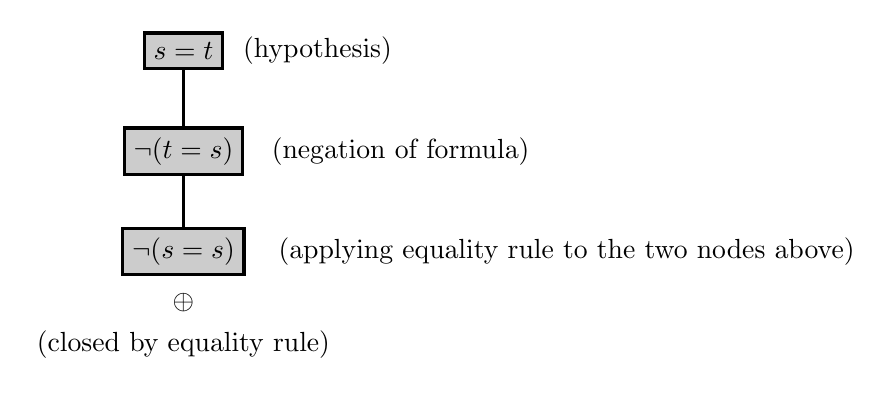
\begin{tikzpicture}[scale=1.275]
        \node (0) at (0, 0)[draw=black, very thick, fill=black!20] {\(s = t\)};
        \node[right of=0, xshift=2em] {(hypothesis)};

        \node (1) at (0, -1)[draw=black, very thick, fill=black!20] {\(\neg(t = s)\)};
        \node[right of=1, xshift=5em] {(negation of formula)};

        \node (2) at (0, -2)[draw=black, very thick, fill=black!20] {\(\neg(s = s)\)};
        \node[right of=2, xshift=11em] {(applying equality rule to the two nodes above)};
        \node [below of=2, yshift=1em] {\(\oplus\)};
        \node [below of=2, yshift=-0.5em] {(closed by equality rule)};

        \draw[black, very thick] (0) -- (1) -- (2);
    \end{tikzpicture}
    \caption{Proving the validity of \(s = t \vdash t = s\) by constructing a predicate tableau using equality rules.}
    \label{fig:Ch05-eq-rule-tableau}
\end{figure}




\subsection{Parents and ancestors}

If a theory \(\Sigma\) in the tableau is dequeued and a new theory \(\Sigma_1\) (and possibly \(\Sigma_2\)) is subsequently enqueued, then \(\Sigma\) is a \emph{parent} of \(\Sigma_1\) and \(\Sigma_2\). We denote this relationship using the function \(P\), defined as follows.
%
\begin{align*}
    P(\Sigma) &= \Sigma' \hspace{2em} \text{if the parent of } \Sigma \text{ is } \Sigma'\\
    P^0(\Sigma) &= \Sigma\\
    P^{n+1} (\Sigma) &= P(P^n (\Sigma))
\end{align*}
%
We say that \(\Sigma'\) is an \emph{ancestor} of \(\Sigma'\) if
%
\[P^n (\Sigma) = \Sigma'\]
%
for some \(n \in \mathbb{N}\). For example, if a tableau is initialised with only one tableau, then that tableau is an ancestor of every theory in the tableau, including itself.



\subsection{Proving the completeness of propositional tableaus}

\begin{theorem}
    The propositional tableau algorithm is complete.
\end{theorem}
\begin{proof}
    To prove completeness, we must show that \(\models\phi\;\implies\;\vdash\phi\), i.e.
    %
    \[\neg\phi \text{ is unsatisfiable } \implies \text{tableau of } \neg\phi \text{ is closed.}\]
    %
    Taking the contrapositive and renaming our variables, we see that this is equivalent to showing that
    %
    \[\text{Tableau of } \phi \text{ does not close} \implies \phi \text{ is satisfiable.}\]

    Assume that the tableau of \(\phi\) does not close. This means that there is some theory in the tableau that, when dequeued, is found to be fully expanded and have no contradictory literals, thus causing \verb|is_satisfiable(|\(\phi\)\verb|)| to return \texttt{True}. We denote this theory by \(\Sigma\).

    Let \(v\) be a valuation where for each propositional letter \(p\), we have
    %
    \[v(p) = \top \iff p \in \Sigma\text{.}\]
    %
    Extending \(v\) to a truth function, it follows that
    %
    \begin{equation}\label{eq:Ch05-all-formulas-in-branch-hold-under-valuation}
        \phi\in\Sigma\implies v(\phi) = \top\tag{*}
    \end{equation}
    %
    for all formulas \(\phi\).

    We shall now prove by induction that the statement
    %
    \[\phi \in P^n (\Sigma) \implies v(\phi) = \top\]
    %
    is true for all \(n \in \mathbb{N}\).

    \textbf{Base case.} For \(n = 0\), we want to show that \(\phi \in P^0 (\Sigma) \implies v(\phi) = \top\). This was already established by equation \eqref{eq:Ch05-all-formulas-in-branch-hold-under-valuation}.

    \textbf{Step case.} Assume for some \(n \in \mathbb{N}\) that the theory \(P^n (\Sigma)\) satisfies \(\phi \in P^n (\Sigma) \implies v(\phi) = \top\). Now consider its parent \(P^{n+1}(\Sigma)\). We know that some expansion rule --- \(\alpha\) or \(\beta\) --- is used to replace some formula in the parent theory \(P^{n+1}(\Sigma)\) with a new formula to form the child theory \(P^n (\Sigma)\).
    %
    \begin{itemize}
        \item If this is an \(\alpha\)-rule, then both formulas \(\alpha_1\) and \(\alpha_2\) will be present in the child theory \(P^n (\Sigma)\). By the induction hypothesis, we have \(v(\alpha_1) = v(\alpha_2) = \top\), so \(v(\alpha) = \top\).
        \item If this is an \(\beta\)-rule, then one of the formulas \(\beta_1\) and \(\beta_2\) will be present in the child theory \(P^n (\Sigma)\). By the induction hypothesis, we have either \(v(\beta_1) = \top\) or \(v(\beta_2) = \top\). In either case we have \(v(\beta) = \top\).
    \end{itemize}
    %
    Since no other formulas are changed when generating \(P^n (\Sigma)\) from \(P^{n+1} (\Sigma)\), we have \(\phi \in P^{n+1} (\Sigma) \implies v(\phi) = \top\), establishing the step case.

    By the principles of induction, we have
    %
    \[\phi \in P^n (\Sigma) \implies v(\phi) = \top\]
    %
    for all \(n \in \mathbb{N}\). Since the initial theory \(\{\phi\}\) is the ancestor of all theories in the tableau, we have \(v(\phi) = \top\), implying satisfiability.
\end{proof}



\subsection{Herbrand structures}

A closed term contains only constant symbols and function symbols, with no free variables. A \emph{Herbrand structure} is a first-order structure \(H = (D, I)\) where
%
\begin{itemize}
    \item the domain \(D\) is defined as the set of closed terms; and
    \item the interpretation \(I = (I_c, I_f, I_p)\) is such that
    %
    \begin{align*}
        I_c (c) &= c \tag{interpret each constant symbol as the symbol itself}\\
        I_f(f^n (d_1, d_2, \cdots, d_n)) &= f^n (d_1, d_2, \cdots, d_n) \tag{interpret each function as the string itself}
    \end{align*}
    %
    and \(I_p\) can be chosen freely.
\end{itemize}
%
It follows that for any closed term \(t\) and any variable assignment\footnote{The variable assignment here is irrelevant since \(t\) is a closed term.} \(A\), we have \([t]^{H, A} = t\).

Herbrand's theorem, which we will not prove here, states that if \(\phi\) does not contain the equality symbol ``='' but is satisfiable in some structure \(S\) and variable assignment \(A\), then it must also be satisfiable in some Herbrand structure \(H\) and variable assignment \(B\).



\subsection{Ranks}

We define the \emph{rank} of a first-order formula \(\phi\), denoted as \(\Rk(\phi)\), as follows.
%
\begin{align*}
    \Rk(P(t_0, t_1, \cdots, t_{k-1})) &= 1\\
    \Rk(\neg\phi) &= \Rk(\phi) + 1\\
    \Rk(\phi\circ\psi) &= \Rk(\phi) + \Rk(\psi) + 1 \tag{where \(\circ\) is a binary connective}\\
    \Rk(\exists x\; \phi) &= \Rk(\phi) + 1\\
    \Rk(\forall x\; \phi) &= \Rk(\phi) + 1
\end{align*}
%
In other words, \(\Rk(\phi)\) is number of nodes in the parse tree of \(\phi\).


\subsection{Proving the completeness of the predicate tableaus}

\begin{lemma}[König's Tree Lemma]
    Let \(T\) be a tree where each node has only finitely many immediate successors. If each branch is of finite length, then the number of nodes in the tree is finite.
\end{lemma}
\begin{proof}
    We prove the contrapositive of the lemma: Assuming that \(T\) has infinitely many nodes, it must contain an infinite branch.

    Assume \(T\) has infinitely many nodes. Let \(P\) be a path starting at the root of \(T\). We say that a node \(n\) in \(T\) is \emph{bottomless} if there are infinitely many nodes below \(n\) in the tree. It follows that the root of \(T\) is bottomless.

    Recall that each node has only finitely many immediate successors. Therefore, the root must only have finitely many (immediate) children. If all of these children are not bottomless, then they must all have finitely many children, which  contradicts the fact that the root is bottomless and has infinitely many nodes beneath it\footnote{This is because the sum of a finite number of finite numbers is finite.}. Hence, the root has at least one bottomless child. Select any one of these bottomless children and append it to the path \(P\).

    This process of selecting a bottomless child of the last node of \(P\) and then adding it to \(P\) can be repeated indefinitely to create an infinite branch.
\end{proof}




\begin{theorem}
    Predicate tableaus are complete.
\end{theorem}
\begin{proof}
    To prove completeness, we must show that \(\models\phi\;\implies\;\vdash\phi\), i.e.
    %
    \[\neg\phi \text{ is unsatisfiable } \implies \text{tableau of } \neg\phi \text{ is closed.}\]
    %
    Taking the contrapositive and renaming our variables, we see that this is equivalent to showing that
    %
    \[\text{Tableau of } \phi \text{ never closes under fair expansion schedule} \implies \phi \text{ is satisfiable.}\]
    %
    Assume the tableau of a formula \(\phi\) never closes under a fair expansion schedule. By the contrapositive of König's Tree Lemma, there must exist an infinite sequence of theories \(\Sigma_0, \Sigma_1, \Sigma_2, \cdots\) from the tableau where \(\Sigma_n = P(\Sigma_{n+1})\). Let \(\Sigma = \cup_{n\in\mathbb{N}}\; \Sigma_n\). Since a fair schedule is used, we have
    %
    \begin{align*}
        \alpha \in \Sigma &\implies \alpha_1 \in \Sigma \text{ and } \alpha_2 \in \Sigma\\
        \beta \in \Sigma &\implies \beta_1 \in \Sigma \text{ or } \beta_2 \in \Sigma\\
        \exists x\; \theta(x) \in \Sigma &\implies \theta(c) \in \Sigma \text{\;\; for some } c\\
        \neg\forall x\; \theta(x) \in \Sigma &\implies \neg\theta(c) \in \Sigma \text{\;\; for some } c\\
        \forall x\; \theta(x) \in \Sigma &\implies \theta(t) \in \Sigma \text{\;\; for all closed terms } t\\
        \neg\exists x\; \theta(x) \in \Sigma &\implies \neg\theta(t) \in \Sigma \text{\;\; for all closed terms } t\text{.} \label{eq:Ch05-fair-schedule-consequence}\tag{*}
    \end{align*}

    Let \(H\) be a Herbrand structure where
    %
    \begin{itemize}
        \item the domain is the set of closed terms in \(\Sigma\);
        \item \(I(t) = t\) for all closed terms \(t\); and
        \item for each \(n\)-ary predicate \(R^n\), let
        %
        \[(t_0, t_1, \cdots, t_{n-1}) \in I(R^n) \iff R^n (t_0, t_1, \cdots, t_{n-1}) \in \Sigma\text{.}\]
    \end{itemize}

    We now prove by complete induction on \(\Rk(\theta)\) that for any sentence \(\theta\), we have
    %
    \[\theta\in\Sigma\implies H \models\theta\text{.}\]
    %
    Strong induction does not require a base case.
    
    \textbf{Step case.} Assume that for some \(n \in\mathbb{N}\), we have
    %
    \[\theta\in\Sigma\implies H \models\theta\]
    %
    for all formulas \(\theta\) with \(\Rk(\theta) < n\). Now consider a new formula with rank \(n\). By equations \eqref{eq:Ch05-fair-schedule-consequence} and our induction hypothesis, the expansions of this new formula --- all of which must have rank strictly less than \(n\) --- are valid in \(H\). It follows that this new formula is also valid in \(H\), completing the step case.

    This shows that \(\theta\in\Sigma\implies H \models\theta\). Since \(\phi\in\Sigma\), we have \(H\models\phi\), so \(\phi\) is satisfiable.
\end{proof}